\documentclass[11pt,a4paper]{article}

\usepackage[utf8]{inputenc}
\usepackage[T1]{fontenc}
\usepackage[french]{babel}
\usepackage[margin=2.4cm]{geometry}
\usepackage{mathpazo}
\usepackage{amsmath,amssymb,mathtools}
\usepackage{graphicx}
\usepackage{booktabs}
\usepackage{caption}
\usepackage{xcolor}
\definecolor{NavyBlue}{RGB}{0,51,102}
\usepackage[colorlinks=true,linkcolor=black,citecolor=black,urlcolor=NavyBlue]{hyperref}
\usepackage{microtype}
\usepackage{titlesec}
\usepackage{fancyhdr}
\usepackage{placeins}
\usepackage{multirow}

\titleformat{\section}{\normalfont\large\bfseries}{\thesection}{0.6em}{}
\titleformat{\subsection}{\normalfont\bfseries}{\thesubsection}{0.6em}{}
\titlespacing*{\section}{0pt}{1.2em}{0.45em}
\titlespacing*{\subsection}{0pt}{0.9em}{0.35em}

\pagestyle{fancy}
\fancyhf{}
\fancyhead[L]{\small\textit{PhaseIndex}}
\fancyhead[R]{\small\thepage}
\renewcommand{\headrulewidth}{0.3pt}

\setlength{\parskip}{0.3em}
\captionsetup{font=small,labelfont=bf}
\frenchbsetup{StandardLists=true}

\newcommand{\Psiv}{\Psi}
\newcommand{\dV}{\Delta V}

\title{\textbf{PhaseIndex}\\[4pt]\Large Un potentiel bistable appris pour la détection des crises de marché~:\\ ce que la physique porte, ce qu'elle décore, et ce qui vacille}
\author{Ahmed Hadirassou\\[2pt]\small Magistère de Physique, Université Paris Cité}
\date{Septembre 2026}

\begin{document}
\maketitle
\thispagestyle{fancy}

\begin{abstract}
\noindent
Nous présentons PhaseIndex, un détecteur de crises de marché dont le c\oe ur est un potentiel de Ginzburg--Landau à deux puits, dont les coefficients sont produits chaque jour par un réseau peu profond, et dans lequel une particule évolue par dynamique de Langevin sous un thermostat lui aussi appris. Sur six fenêtres de test causales couvrant 2007--2023, le modèle atteint un ROC-AUC moyen de $0{,}894$ et surpasse quatre détecteurs classiques (VIX, GARCH, chaîne de Markov cachée, règle de tendance) sur la précision, la calibration et le F1, tout en étant devancé par la règle de tendance sur le seul ROC-AUC. Plutôt que de nous arrêter à ce tableau, nous avons soumis l'architecture à un programme d'ablations pré-enregistrées destiné à établir ce que chaque composante physique apporte réellement. Les résultats sont contrastés et nous les rapportons tels quels~: le réseau qui pilote le terme de brisure de symétrie est remplaçable par un unique scalaire appris sans perte mesurable~; figer l'ensemble des paramètres physiques à six constantes ne coûte rien sur le classement mais coûte sur la précision et sur une crise particulière~; l'encodeur peut être rendu linéaire~; le restreindre à la volatilité seule détruit la calibration. Les constantes vers lesquelles converge le modèle figé --- hauteur de barrière, friction, température --- sont remarquablement stables sur les six fenêtres d'entraînement. Enfin, lire le modèle par sa physique plutôt que par sa seule tête de sortie (taux d'échappement de Kramers, variance glissante de la jauge) fournit des signaux qui détectent le \emph{début} des crises là où la sortie apprise échoue, et un ensemble de rangs sans paramètre gagne $+0{,}02$ de ROC-AUC et $+0{,}04$ à $+0{,}07$ de Transition-AUC. Pris ensemble, ces résultats convergent avec la thèse de Guttal \emph{et al.} selon laquelle les krachs financiers ne présentent pas de ralentissement critique~: le paysage énergétique ne s'aplatit pas, le système vacille. Nous discutons franchement les limites du travail --- six crises, fenêtres emboîtées, un seul marché.
\end{abstract}

\section{Introduction}

Il existe deux façons de construire un détecteur de crises financières. La première consiste à empiler des descripteurs et à laisser un modèle statistique en tirer ce qu'il peut~; elle donne souvent de bons chiffres et peu de compréhension. La seconde consiste à postuler un mécanisme, à l'écrire sous forme d'équations, et à n'apprendre que ce que le mécanisme ne fixe pas~; elle donne parfois de moins bons chiffres, mais elle permet de poser des questions. Ce travail relève de la seconde approche, et l'essentiel de ce qui suit est consacré aux questions plutôt qu'aux chiffres.

Le mécanisme postulé n'est pas nouveau. Depuis Bouchaud et Cont~\cite{bouchaud1998}, on sait qu'une équation de Langevin dans un potentiel non linéaire reproduit plusieurs faits stylisés des marchés, et l'image d'un système bistable --- un puits de calme, un puits de stress, une barrière entre les deux --- traverse la littérature depuis. Halperin et Dixon~\cite{halperin2019} ont fait de la brisure de symétrie d'un tel potentiel une théorie des défauts~; Wand \emph{et al.}~\cite{wand2024} ont estimé des potentiels de Langevin sur des séries financières et y ont trouvé des points fixes stables~; Rinn \emph{et al.}~\cite{rinn2015} ont montré que la dynamique des corrélations de marché se lit comme un système quasi stationnaire. Notre contribution n'est pas dans le mécanisme, elle est dans l'estimateur~: là où ces travaux ajustent un potentiel par fenêtre, nous laissons un réseau produire ses coefficients \emph{chaque jour}, à partir de descripteurs lents, et nous apprenons le thermostat en même temps.

Cette liberté a un prix, et c'est ce prix que nous avons voulu mesurer. Un modèle qui apprend un potentiel par jour peut apprendre un potentiel qui ne sert à rien --- un décor physique posé sur ce qui est, en réalité, un classifieur ordinaire. La question n'est pas rhétorique~: nous avons construit, testé et rejeté quatre extensions de l'architecture avant d'arriver à la version présentée ici, et chacune a échoué de la même manière, en ajoutant de la liberté qui déstabilisait ce que le modèle avait déjà appris. Il était donc légitime de se demander si la physique déjà en place était elle-même nécessaire.

Nous avons répondu par une série d'ablations dont la grille de lecture a été fixée avant de lancer les calculs. Chacune retire une composante et mesure ce qui reste, en tenant compte du bruit inter-graines, que nous avons pris soin d'enregistrer partout. La section~\ref{sec:ablations} présente ce programme et ses résultats, qui ne sont pas ceux qu'un auteur souhaiterait~: une part importante de ce que le modèle apprend jour après jour est décorative pour le classement. Mais ce n'est pas tout ce qu'ils disent, et la section~\ref{sec:physics} montre que la physique, lue autrement --- par le taux d'échappement de Kramers, par la variance de la jauge --- porte une information que la tête de sortie apprise ne capture pas, en particulier au moment où une crise commence.

Le fil qui relie ces résultats est une question de mécanisme que la littérature des transitions critiques pose depuis Scheffer \emph{et al.}~\cite{scheffer2009}~: un système qui approche d'un basculement le signale-t-il en ralentissant, parce que son puits s'aplatit, ou en vacillant, parce que le bruit le pousse par intermittence de l'autre côté d'une barrière qui, elle, ne bouge pas~? Guttal \emph{et al.}~\cite{guttal2016} ont montré que les krachs du Dow Jones ne présentent pas la signature du ralentissement. Nos ablations disent la même chose de l'intérieur du modèle, et nos signaux de vacillement la confirment de l'extérieur. Nous ne prétendons pas clore la question~; nous apportons trois observations indépendantes qui pointent dans le même sens.

Le reste de l'article est organisé comme suit. La section~\ref{sec:related} situe le travail. La section~\ref{sec:model} décrit le modèle et la section~\ref{sec:protocol} le protocole d'évaluation. La section~\ref{sec:results} donne les résultats principaux et la comparaison aux détecteurs classiques. La section~\ref{sec:audit} vérifie que le modèle apprend un mécanisme et non des dates. La section~\ref{sec:ablations} présente le programme d'ablations, la section~\ref{sec:physics} les signaux physiques, et la section~\ref{sec:discussion} ce que l'ensemble suggère. La section~\ref{sec:limits} liste ce que nous ne savons pas.

\section{Travaux voisins et positionnement}
\label{sec:related}

\paragraph{Potentiels de Langevin en finance.} L'idée de représenter un marché par une particule dans un potentiel remonte à Bouchaud et Cont~\cite{bouchaud1998}, qui montrent qu'une non-linéarité dans la réponse des agents suffit à produire des krachs. Halperin et Dixon~\cite{halperin2019} construisent un potentiel quartique dont la brisure de symétrie représente le défaut~; Wand \emph{et al.}~\cite{wand2024} estiment directement le potentiel et ses points fixes sur des indices. Notre potentiel a la même forme que celui de ces travaux. Ce qui change est l'estimateur --- un réseau produit les coefficients chaque jour --- et l'ajout d'un thermostat appris. Nous verrons que cette liberté supplémentaire est en grande partie inutile, ce qui, rétrospectivement, plaide pour l'approche plus sobre de nos prédécesseurs.

\paragraph{Le modèle de Chiarella et la tendance.} La compétition entre agents suiveurs de tendance et agents de valeur, formalisée par Chiarella~\cite{chiarella1992}, produit naturellement une bimodalité~: le marché est plus souvent sur- ou sous-évalué que correctement évalué. Majewski \emph{et al.}~\cite{majewski2020} ont calibré ce modèle sur plusieurs classes d'actifs~; Kurth, Majewski et Bouchaud~\cite{kurth2025excess} ont étendu la calibration aux dérives de long terme, et Kurth et Bouchaud~\cite{kurth2025chiarella} ont établi les distributions stationnaires du modèle et les conditions de la bimodalité. Nous empruntons à cette lignée la forme du terme de tendance --- une moyenne exponentielle des rendements passés, saturée par une tangente hyperbolique --- que nous utilisons comme terme de brisure de symétrie du potentiel.

\paragraph{Signaux précurseurs et transitions critiques.} Scheffer \emph{et al.}~\cite{scheffer2009} ont proposé que les systèmes proches d'une bifurcation présentent un ralentissement critique, visible dans l'autocorrélation et la variance. Wang \emph{et al.}~\cite{wang2012} et Dakos \emph{et al.}~\cite{dakos2013} ont décrit un mécanisme alternatif, le vacillement, dans lequel un système bistable sous fort bruit traverse par intermittence vers l'autre état avant de s'y installer. Perretti et Munch~\cite{perretti2012} ont montré que les indicateurs de ralentissement échouent sous des niveaux de bruit réalistes. En finance, Guttal \emph{et al.}~\cite{guttal2016} n'ont trouvé aucun ralentissement critique avant les krachs américains de 1929, 1987, 2000 et 2008, tout en observant une montée de la variance, et Diks \emph{et al.}~\cite{diks2019} ont exprimé un scepticisme voisin. Notre modèle est en position d'interroger ce débat de l'intérieur, parce qu'il apprend séparément la forme du puits et l'intensité du bruit.

\paragraph{Log-périodicité.} Le cadre de Sornette~\cite{sornette2003,johansen1999} prédit les krachs par une accélération log-périodique du prix. Il est directement pertinent mais nous ne l'implémentons pas~: son ajustement non linéaire est notoirement instable et ses propres auteurs rapportent des fausses alertes historiques. Nous le citons comme approche concurrente, non comme composante.

\paragraph{Détecteurs classiques.} Nous comparons à quatre références~: le niveau du VIX~\cite{whaley2000}, une volatilité conditionnelle GARCH(1,1)~\cite{bollerslev1986}, un modèle à changement de régime de Hamilton~\cite{hamilton1989}, et une règle de tendance sur moyenne mobile à 200 jours~\cite{faber2007}, apparentée au momentum de séries temporelles~\cite{moskowitz2012}. La géométrie des corrélations~\cite{sandhu2016} et la topologie persistante~\cite{topological2025} sont d'autres approches physiques récentes que nous ne comparons pas ici.

\section{Le modèle}
\label{sec:model}

\subsection{Descripteurs et séparation des échelles}

Le modèle lit chaque jour un vecteur de 204 descripteurs calculés à partir des prix du S\&P~500 et d'un panier d'instruments annexes (ETF sectoriels, obligations, matières premières, indice VIX), tous connus au soir du jour $t$. Ces descripteurs sont séparés en deux blocs selon l'échelle de temps qu'ils encodent. Le bloc \emph{lent} (80 descripteurs~: statistiques d'ordre supérieur, macro) alimente le potentiel~; le bloc \emph{rapide} (124 descripteurs~: volatilité, momentum, structure de marché, vitesse) alimente l'état de la particule et le thermostat. Cette séparation est un choix de modélisation, non une propriété des données~: elle exprime l'hypothèse qu'un paysage énergétique change lentement et qu'une position dans ce paysage change vite. Nous verrons en section~\ref{sec:ablations} que l'hypothèse n'est qu'à moitié confirmée.

\subsection{Le potentiel}

Dans un espace latent de dimension $d=4$, la particule de position $\mathbf{z}$ évolue dans le potentiel
\begin{equation}
V(\mathbf{z}) \;=\; a\,\lVert\mathbf{z}\rVert^{4} \;-\; b\,\lVert\mathbf{z}\rVert^{2} \;+\; c\,\bar{z},
\qquad \bar z = \tfrac{1}{d}\textstyle\sum_i z_i ,
\label{eq:potential}
\end{equation}
dont les deux premiers termes forment un puits double radial --- minimum sur la sphère $\lVert\mathbf z\rVert^2 = b/2a$, barrière en $\mathbf z = 0$ de hauteur $\dV = b^2/4a$ --- et dont le troisième brise la symétrie en inclinant le paysage dans une direction. Les coefficients $(a,b,c)$ sont produits chaque jour par un réseau à une couche cachée de 32 unités lisant le bloc lent, avec $a,b>0{,}1$ par une fonction softplus et $c\in[-2,2]$ par une tangente hyperbolique. C'est la forme de Ginzburg--Landau, la même que celle des références citées plus haut~; ce qui diffère est que ses coefficients bougent au jour le jour.

\subsection{Dynamique}

La particule suit une équation de Langevin sous-amortie avec mémoire, intégrée par un schéma de Verlet~\cite{verlet1967} à $N=6$ pas de $\delta t = 0{,}1$~:
\begin{align}
\mathbf p_{n+1} &= (1-\gamma)\,\mathbf p_n \;-\; \delta t\,\nabla V(\mathbf z_n) \;+\; \delta t\,\mathbf f_{\mathrm{ext}} \;-\; \varphi\,\mathbf s_n \;+\; \sqrt{2\gamma T\,\delta t}\;\boldsymbol\xi_n, \\
\mathbf z_{n+1} &= \mathbf z_n + \delta t\,\mathbf p_{n+1}, \qquad
\mathbf s_{n+1} = \alpha\,\mathbf s_n + (1-\alpha)\,\mathbf p_{n+1}.
\end{align}
La friction $\gamma\in(0,1)$, la température $T\in[0{,}005,\,0{,}12]$, la force externe $\mathbf f_{\mathrm{ext}}$, l'intensité de mémoire $\varphi$ et son taux d'oubli $\alpha$ sont produits chaque jour par un second réseau lisant le bloc rapide, de même que l'état initial $(\mathbf z_0,\mathbf p_0)$. Le terme de mémoire $\mathbf s$ est un noyau de Mori--Zwanzig~\cite{mori1965,zwanzig1961} réduit à une exponentielle. Le bruit thermique $\boldsymbol\xi$ n'est injecté qu'à l'entraînement~; l'inférence est déterministe. La relation $\sigma^2 = 2\gamma T\delta t$ est celle de fluctuation--dissipation à l'équilibre~; nous verrons qu'elle est violée, et qu'il est plus instructif de mesurer la violation que de la corriger.

L'état est \emph{propagé} d'un jour au suivant~: la position finale $\mathbf z_N$ du jour $t$ sert d'état initial au jour $t+1$, ce qui rend l'inférence séquentielle et causale.

\subsection{Sortie et entraînement}

Une tête de lecture à une couche cachée de 16 unités transforme $(\mathbf z_N,\mathbf p_N)$ en une jauge $\Psiv\in[0,1]$. Le modèle est entraîné contre des étiquettes \emph{douces}~: chaque épisode de crise, daté à la main, est converti en une bosse gaussienne centrée sur l'épisode, ce qui lisse les frontières temporelles arbitraires. La perte est une entropie croisée asymétrique qui pénalise trois fois plus une crise manquée qu'une fausse alerte ($K=3$). L'optimisation utilise Adam sur 45 époques~; nous rapportons en section~\ref{sec:audit} pourquoi ce calendrier fixe est un défaut.

Treize épisodes de crise sont datés sur 1994--2023~: la crise obligataire de 1994, la crise asiatique, LTCM, le 11~septembre, les scandales comptables de 2002, l'été 2007, l'effondrement de 2008--2009, la crise de la dette européenne en deux temps (2010, 2011), la correction chinoise de 2015, le quatrième trimestre 2018, le choc COVID et le marché baissier de 2022. Ce n'est pas beaucoup. C'est l'histoire disponible.

\section{Protocole d'évaluation}
\label{sec:protocol}

\subsection{Validation causale}

Toute évaluation suit un schéma de marche en avant à six plis. Pour chaque pli, le modèle est entraîné sur toutes les données jusqu'à une date $t_0$, la température de calibration est ajustée sur les 504 derniers jours de cette fenêtre, et le modèle est testé sur les deux ou trois années suivantes sans jamais les avoir vues. Les fenêtres de test sont 2007--2009, 2011--2012, 2015--2016, 2018--2019, 2020--2021 et 2022--2023, choisies pour contenir chacune au moins un épisode de crise. Les fenêtres d'entraînement sont \emph{emboîtées}~: chaque pli contient tout ce que le précédent contenait. Nous reviendrons sur ce que cela implique.

Chaque configuration est entraînée avec cinq graines aléatoires, et nous rapportons à la fois la performance de l'ensemble et celle de chaque graine. Ce dernier point est essentiel~: l'écart-type inter-graines est, sur certains plis, plus grand que la plupart des effets que nous cherchons à mesurer, et nous nous imposons la règle suivante tout au long de l'article --- \emph{un écart entre deux configurations qui ne dépasse pas l'écart-type inter-graines du pli concerné n'est pas rapporté comme un effet}.

\subsection{Métriques}

Nous rapportons le ROC-AUC, le PR-AUC --- plus informatif sur une classe rare~\cite{saito2015} --- le F1 à un seuil fixé une fois pour toutes par le rapport d'asymétrie de la perte ($\tau = 1/(1+K) = 0{,}25$), l'erreur de calibration attendue (ECE~\cite{guo2017}) après ajustement de température, et le temps d'avance, défini comme le nombre de jours entre le premier franchissement du seuil et le début daté de l'épisode.

Nous ajoutons une métrique qui n'est pas standard et que nous devons justifier. Le ROC-AUC sur une fenêtre complète récompense un détecteur qui étiquette correctement le milieu d'un marché baissier de deux ans, ce qui est facile~; un détecteur qui ne remarque une crise que trois semaines après son début peut encore obtenir un excellent score. Nous définissons la \emph{Transition-AUC} comme le ROC-AUC restreint, pour chaque crise, aux 60 jours ouvrés qui la précèdent et aux 20 premiers jours qui la suivent, agrégés sur les crises de la fenêtre. Cette métrique a été proposée dans l'espoir qu'elle avantagerait notre modèle. Elle est rapportée quel que soit son verdict, et nous verrons qu'il n'est pas uniformément favorable.

\subsection{Pré-enregistrement}

Chaque ablation de la section~\ref{sec:ablations} a été précédée d'une grille de lecture écrite avant le calcul, indiquant ce que chaque issue possible signifierait. Nous avons procédé ainsi parce que, sur six crises, la tentation de trouver après coup une lecture favorable à n'importe quel résultat est forte, et qu'elle est exactement le mécanisme que Gelman et Loken~\cite{gelman2013} appellent le jardin des sentiers qui bifurquent. Les grilles sont reproduites dans le texte au moment où elles ont servi.

\section{Résultats principaux}
\label{sec:results}

\subsection{Performance en marche en avant}

Le tableau~\ref{tab:main} donne les résultats du modèle complet sur les six plis. Le ROC-AUC moyen est de $0{,}894\pm0{,}056$, le PR-AUC de $0{,}753\pm0{,}181$. La dispersion du second est frappante, et elle raconte quelque chose de vrai~: le modèle sépare presque parfaitement les crises profondes (2008, la dette européenne, COVID) et beaucoup moins bien les corrections modérées (2015, 2018). Nous avions écrit dans une version antérieure que le modèle atteignait un ROC-AUC supérieur à $0{,}94$ sur les paniques rapides~; le pli 2008 est à $0{,}889$ et cette affirmation était fausse. La formulation correcte est un ordre de sévérité~: rappel quasi total sur les épisodes profonds, partiel sur les épisodes modérés.

\begin{table}[htbp]
\centering\small
\caption{Marche en avant, modèle complet, ensemble de cinq graines. $\dagger$~: la queue de calibration ne contient aucun jour de crise, la température vaut $1$ et l'ECE n'est pas comparable. $\ddagger$~: moyenne sur les plis 2, 5, 6 seulement.}
\label{tab:main}
\begin{tabular}{lcccccl}
\toprule
Pli & ROC-AUC & PR-AUC & F1 & ECE & AUC entraînement & Avance (jours) \\
\midrule
1 (2007--09) & 0,889 & 0,819 & 0,604 & 0,150$^\dagger$ & 0,989 & 123, 126 \\
2 (2011--12) & 0,985 & 0,951 & 0,853 & 0,012 & 0,976 & aucune \\
3 (2015--16) & 0,847 & 0,696 & 0,341 & 0,191$^\dagger$ & 0,983 & 88 \\
4 (2018--19) & 0,822 & 0,389 & 0,464 & 0,157$^\dagger$ & 0,983 & 125 \\
5 (2020--21) & 0,948 & 0,884 & 0,742 & 0,060 & 0,977 & aucune \\
6 (2022--23) & 0,870 & 0,781 & 0,705 & 0,057 & 0,979 & 33 \\
\midrule
Moyenne & 0,894 & 0,753 & 0,767$^\ddagger$ & 0,043$^\ddagger$ & 0,981 & 99$^\ddagger$ \\
\bottomrule
\end{tabular}
\end{table}

Deux colonnes méritent un commentaire. L'AUC d'entraînement est de $0{,}981$ en moyenne~: le modèle mémorise sa fenêtre d'entraînement sans difficulté, et l'écart avec le test ($+0{,}087$ en moyenne) est la première raison de la section~\ref{sec:audit}. Le temps d'avance, lorsqu'il existe, est long --- trois à quatre mois avant 2008, 2015 et 2018 --- mais il n'existe pas pour deux crises sur sept, la dette européenne et le COVID, où le modèle ne franchit le seuil qu'après le début daté. Un détecteur qui anticipe certaines crises de quatre mois et en manque d'autres entièrement n'est pas un détecteur uniforme, et nous ne le présentons pas comme tel.

\subsection{Comparaison aux détecteurs classiques}

Le tableau~\ref{tab:baselines} compare, sur les mêmes plis et le même protocole, quatre détecteurs qui n'ont ni potentiel ni thermostat. Le résultat est mitigé et nous le donnons tel quel. PhaseIndex mène sur le PR-AUC, le F1 et la calibration. La règle de tendance à 200 jours le devance sur le ROC-AUC, de $0{,}027$, ce qui est plus que la moitié de l'écart-type inter-plis. Une moyenne mobile classe donc mieux les jours que notre modèle~; notre modèle est plus précis sur la classe qui compte et bien mieux calibré. Selon l'usage, l'un ou l'autre est préférable, et nous n'avons pas de raison de dire que le nôtre l'est en général.

\begin{table}[htbp]
\centering\small
\caption{Détecteurs classiques, six plis, même protocole. $\ddagger$~: plis 2, 5, 6 seulement.}
\label{tab:baselines}
\begin{tabular}{lcccc}
\toprule
Modèle & ROC-AUC & PR-AUC & F1$^\ddagger$ & ECE$^\ddagger$ \\
\midrule
PhaseIndex & 0,894 $\pm$ 0,056 & \textbf{0,753} & \textbf{0,767} & \textbf{0,043} \\
Tendance MM200 & \textbf{0,921} $\pm$ 0,051 & 0,723 & 0,737 & 0,091 \\
Niveau du VIX & 0,868 $\pm$ 0,077 & 0,663 & 0,359 & 0,198 \\
GARCH(1,1) & 0,858 $\pm$ 0,079 & 0,666 & 0,473 & 0,117 \\
Markov caché & 0,840 $\pm$ 0,081 & 0,544 & 0,510 & 0,072 \\
\bottomrule
\end{tabular}
\end{table}

Ce tableau a orienté la suite du travail. Si une moyenne mobile fait aussi bien sur le classement, la question n'est plus \og le modèle est-il bon~? \fg{} mais \og d'où vient l'avantage de la moyenne mobile, et qu'est-ce que le modèle fait que la moyenne mobile ne fait pas~? \fg{}. Les sections~\ref{sec:ablations} et~\ref{sec:physics} tentent d'y répondre.

\section{Le modèle apprend-il un mécanisme~?}
\label{sec:audit}

Avant de demander ce que la physique apporte, il faut établir que le modèle apprend autre chose que les dates des crises de son entraînement. Cinq diagnostics distincts convergent, et l'un d'eux révèle un défaut que nous rapportons plutôt que de le corriger discrètement.

\paragraph{Permutation des étiquettes.} Sur les plis 1 à 4, nous avons réentraîné le modèle dix fois avec des étiquettes redistribuées aléatoirement dans le temps (figure~\ref{fig:permutation}). Le ROC-AUC réel moyen est de $0{,}884$~; la distribution nulle est centrée à $0{,}397\pm0{,}112$. L'écart est de $4{,}35$ écarts-types. Le centre de la distribution nulle est \emph{sous} $0{,}5$, ce qui a d'abord surpris~: c'est que le modèle, même entraîné sur des étiquettes fausses, continue de réagir aux vrais épisodes de stress par ses descripteurs de volatilité, et que ces réactions tombent, par construction, sur des jours étiquetés au hasard, donc majoritairement hors crise. Le signal est réel~; il n'est pas une mémoire des dates.

\begin{figure}[htbp]
\centering
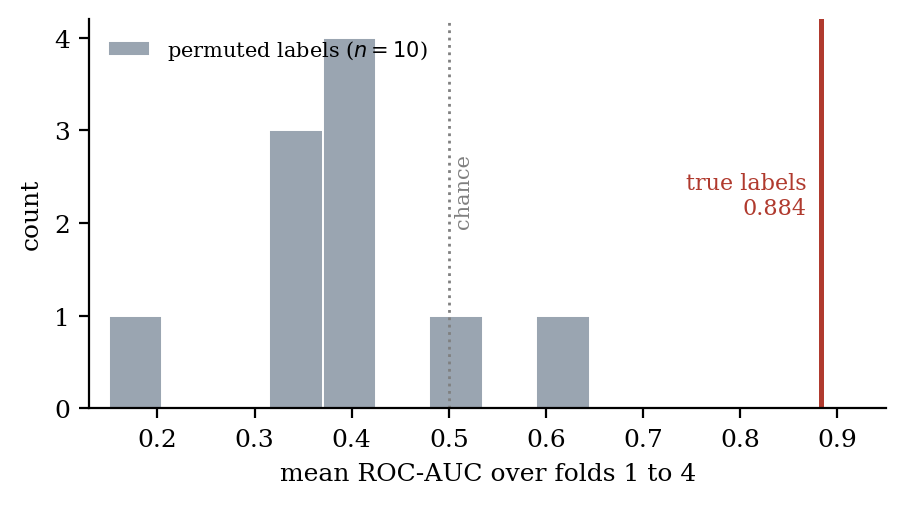
\includegraphics[width=0.6\textwidth]{figures/12_permutation.png}
\caption{Test de permutation, plis 1 à 4, dix tirages. Le ROC-AUC réel (trait vertical) est à $4{,}35$ écarts-types de la distribution nulle.}
\label{fig:permutation}
\end{figure}

\paragraph{Sensibilité aux hyperparamètres et à la taille du jeu.} Faire varier la dimension latente entre 3 et 5 déplace le ROC-AUC dans une plage de $0{,}010$. Entraîner sur 50, 75 et 100~\% de la fenêtre donne $0{,}991$, $0{,}994$ et $0{,}987$~: aucune amélioration monotone, ce qui indique que le modèle n'est pas limité par la quantité de données mais par ce qu'elles contiennent.

\paragraph{Ablation par groupe de descripteurs.} En remplaçant tour à tour chaque groupe par sa moyenne d'entraînement, seul le groupe volatilité coûte plus que le bruit ($-0{,}019$)~; statistiques, momentum, macro et vitesse coûtent chacun moins de $0{,}01$. Le modèle est, pour l'essentiel, un détecteur de volatilité habillé. Ce constat, fait sur un pli et une graine, sera mis à l'épreuve à pleine échelle en section~\ref{sec:minimal}.

\paragraph{Un défaut du calendrier d'entraînement.} La figure~\ref{fig:early} montre le ROC-AUC de test à chaque époque, pour chaque pli. Le calendrier fixe de 45 époques dépasse l'optimum sur cinq plis sur six, laissant en moyenne $0{,}022$ de ROC-AUC sur la table. Nous devons immédiatement corriger ce que ce chiffre suggère~: c'est un gain \emph{oracle}, obtenu en choisissant le meilleur point de contrôle en regardant le jeu de test. Un critère honnête d'arrêt précoce, fondé sur la perte de validation de la queue de calibration, ne récupère que $+0{,}0001$ sur les plis où nous avons pu le mesurer (figure~\ref{fig:trainval})~: le minimum de la perte de validation ne coïncide pas avec le maximum du ROC-AUC de test. Le défaut est réel, sa correction réaliste est presque sans effet, et nous laissons le calendrier tel quel plutôt que d'y ajouter un mécanisme qui ne change rien.

\begin{figure}[htbp]
\centering
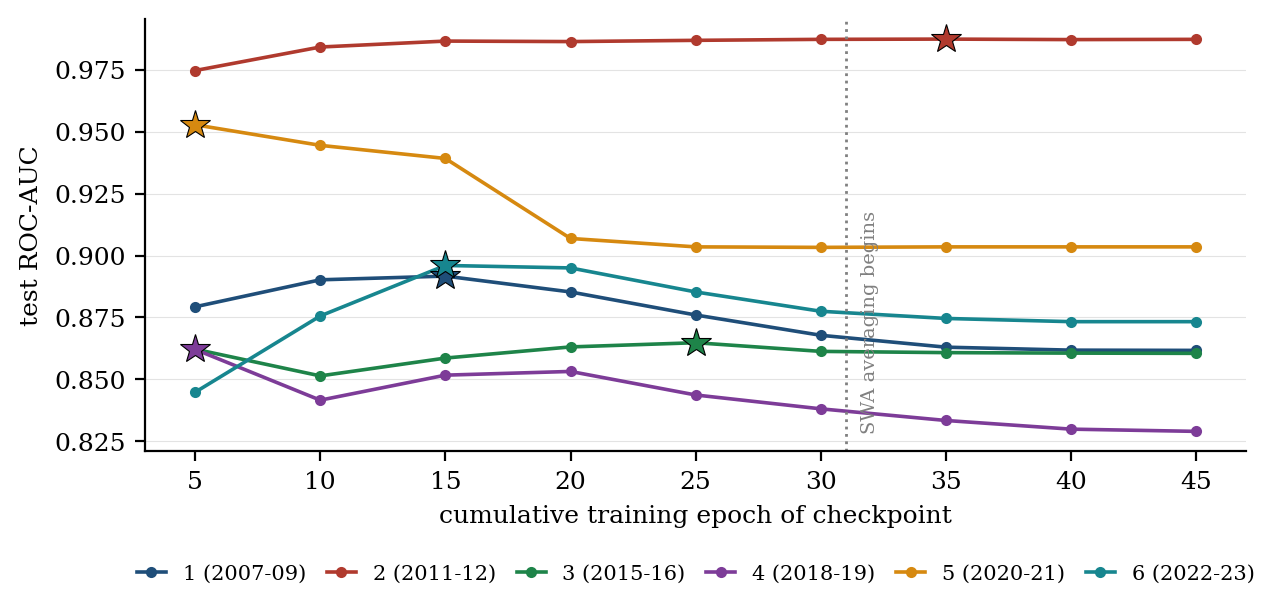
\includegraphics[width=0.92\textwidth]{figures/10_early_stopping.png}
\caption{ROC-AUC de test par époque, une graine, six plis. Le trait pointillé marque l'époque 45. Le meilleur point est marqué~; sa distance à l'époque 45 est le gain oracle.}
\label{fig:early}
\end{figure}

\begin{figure}[htbp]
\centering
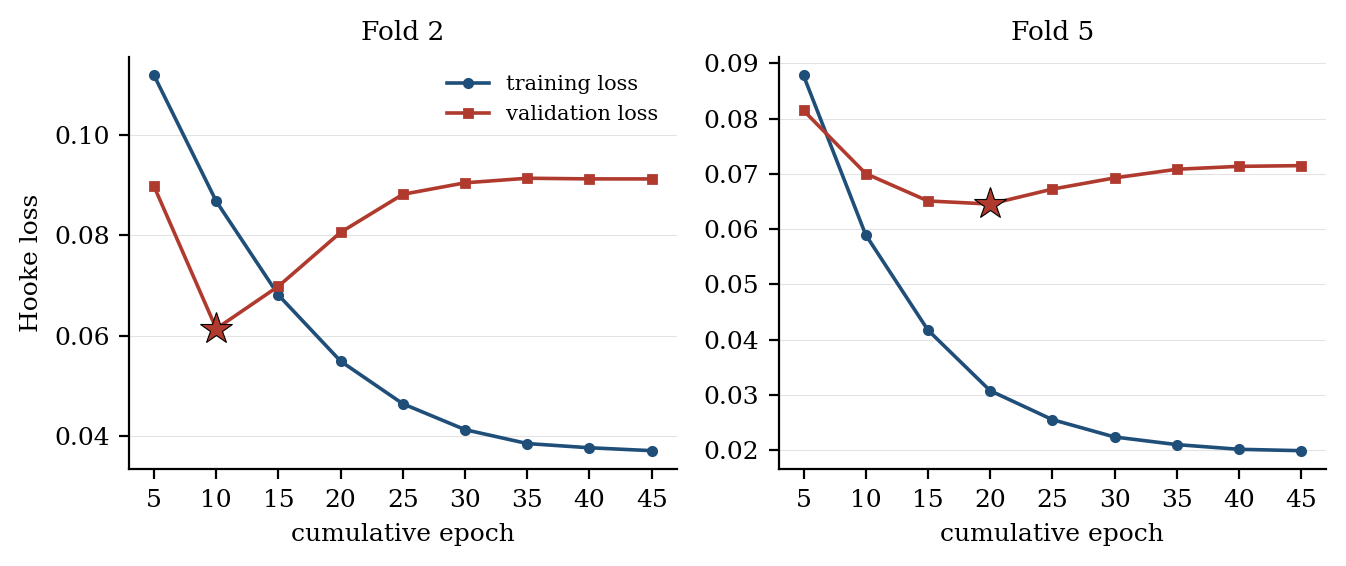
\includegraphics[width=0.86\textwidth]{figures/11_train_val.png}
\caption{Perte d'entraînement et de validation, plis 2 et 5. La perte de validation remonte après son minimum, mais ce minimum n'est pas le maximum du ROC-AUC de test.}
\label{fig:trainval}
\end{figure}

\FloatBarrier
\section{Ce que la physique porte~: un programme d'ablations}
\label{sec:ablations}

Nous avons établi que le modèle apprend un signal. Nous demandons maintenant quelle part de son architecture physique est nécessaire à ce signal. Trois ablations se suivent, chacune retirant une composante, chacune précédée d'une grille de lecture fixée avant le calcul. Toutes utilisent le protocole complet~: six plis, cinq graines, scores par graine enregistrés.

\subsection{Le terme de brisure de symétrie}
\label{sec:tilt}

La règle de tendance nous devance sur le ROC-AUC. Une hypothèse simple est que le modèle manque d'information de tendance~: ses descripteurs de momentum vont jusqu'à 120 jours, la moyenne mobile qui le bat en utilise 200. Une seconde hypothèse, plus intéressante, est que le modèle a l'information mais pas la structure pour l'utiliser~: le coefficient $c$ de l'équation~\eqref{eq:potential} est produit par un réseau qui doit découvrir seul que la tendance devrait incliner le paysage. Suivant Chiarella~\cite{chiarella1992} et la forme utilisée par Kurth et Bouchaud~\cite{kurth2025chiarella}, nous construisons un signal de tendance $M_t$, moyenne exponentielle des rendements journaliers d'horizon $\tau=200$ jours fixé \emph{a priori} pour coïncider avec celui de la règle concurrente, et nous testons quatre variantes~:
\begin{itemize}\setlength\itemsep{0pt}
\item \textbf{v2}~: $c = 2\tanh(\mathbf w\cdot\mathbf h)$, le réseau seul --- le modèle déployé, bit pour bit~;
\item \textbf{horizon}~: le même réseau, recevant $M_t$ comme entrée supplémentaire, sans structure imposée~;
\item \textbf{physics}~: $c = 2\tanh(g\,z(M_t))$, un unique scalaire appris $g$, le réseau débranché de $c$~;
\item \textbf{coupled}~: $c = 2\tanh(g\,z(M_t) + \mathbf w\cdot\mathbf h)$, les deux.
\end{itemize}
Les quatre branches sont \emph{emboîtées}~: coupled avec $g=0$ redonne v2, coupled avec $\mathbf w=0$ redonne physics. Elles ont le même nombre de paramètres à un près et la même plage atteignable pour $c$. Le scalaire $g$ absorbe amplitude, pente et signe~; nous avons refusé de fixer le signe à la main parce que rien dans le potentiel ne dit quel bassin est celui de la crise --- c'est la tête de lecture, apprise, qui le décide.

La grille de lecture était la suivante. Si horizon bat coupled, le modèle n'avait pas besoin de physique, seulement d'un horizon plus long. Si physics égale coupled, le réseau était inutile pour structurer l'asymétrie et le scalaire suffit. Si coupled bat les deux, le couplage hybride apporte quelque chose que ni l'information seule ni la structure seule n'apportent.

\begin{figure}[htbp]
\centering
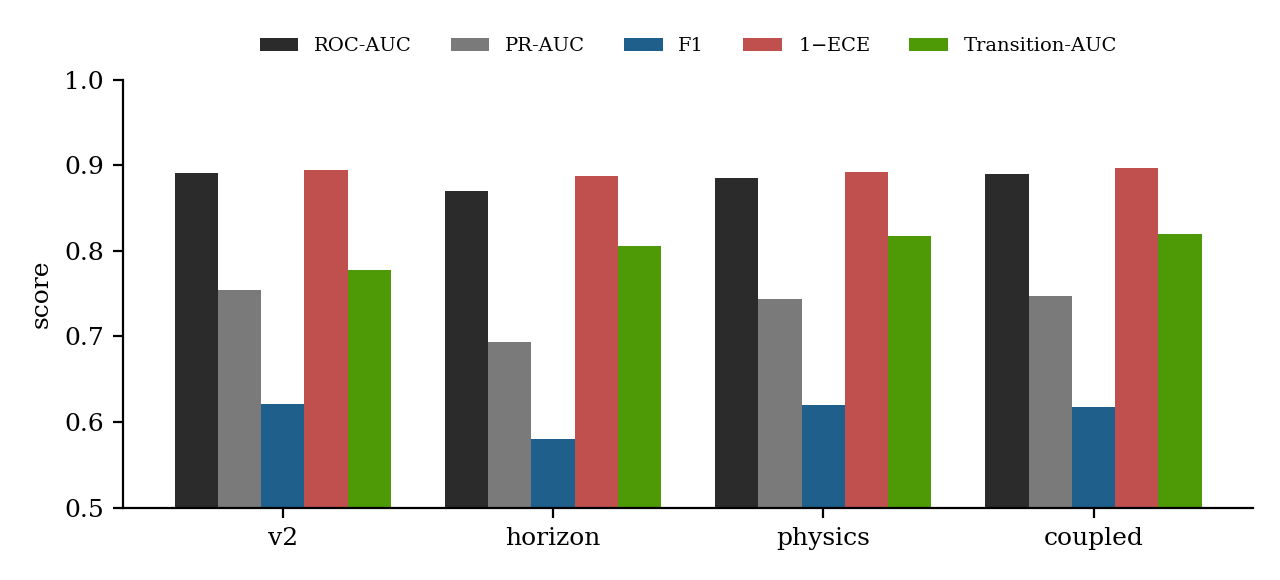
\includegraphics[width=0.9\textwidth]{figures/13_tilt_ablation.png}
\caption{Ablation du terme de brisure de symétrie, quatre branches, moyennes sur six plis et cinq graines.}
\label{fig:tilt}
\end{figure}

La figure~\ref{fig:tilt} donne le résultat, et c'est la deuxième issue qui s'est produite. Physics et coupled sont indiscernables sur chacun des six plis, chaque écart de ROC-AUC étant inférieur à l'écart-type inter-graines du pli (le plus grand, $+0{,}037$ sur le pli 6, contre un bruit de $0{,}062$). Le réseau $\mathbf w\cdot\mathbf h$ avait toute latitude pour dominer~; il n'a rien ajouté de mesurable au-delà de $g$. Horizon, lui, est clairement battu~: coupled le dépasse au-delà du bruit sur les plis 1 et 4. L'information brute de tendance, donnée au réseau sans structure, ne suffit pas et dégrade même le classement. Le troisième scénario n'a pas eu lieu.

Ce que cela veut dire est simple~: le terme de brisure de symétrie peut être écrit $c = 2\tanh(g\,z(M_t))$, un scalaire appris et une forme fonctionnelle empruntée à Chiarella, sans perte. C'est un résultat de parcimonie, et il déplace un morceau de l'architecture du côté de la physique. Il a aussi un effet que nous n'attendions pas~: physics et coupled gagnent tous deux sur la Transition-AUC ($+0{,}040$ et $+0{,}042$ en moyenne), et ce gain est concentré presque entièrement sur le pli 4 ($+0{,}187$ et $+0{,}176$). Nous reviendrons sur ce pli.

\subsection{Ce qui bouge~: potentiel ou thermostat}
\label{sec:mechanism}

Le modèle apprend séparément, chaque jour, la forme du puits par $(a,b)$ et l'intensité du bruit par $(\gamma,T)$. Le débat que nous avons rappelé en section~\ref{sec:related} oppose deux mécanismes de basculement~: un puits qui s'aplatit (ralentissement critique) ou un bruit qui monte pendant que le puits reste en place (transition stochastique, vacillement). Guttal \emph{et al.}~\cite{guttal2016} ont tranché en faveur du second sur le Dow Jones. Notre modèle permet de poser la question de l'intérieur, en gelant l'un des deux mécanismes et en laissant l'autre libre~:
\begin{itemize}\setlength\itemsep{0pt}
\item \textbf{LL}~: potentiel par jour, thermostat par jour (référence)~;
\item \textbf{FL}~: potentiel \emph{figé} à deux scalaires appris $(a,b)$, thermostat par jour~;
\item \textbf{LF}~: potentiel par jour, thermostat \emph{figé} à deux scalaires appris $(\gamma,T)$~;
\item \textbf{FF}~: les deux figés.
\end{itemize}
\og Figé \fg{} signifie un scalaire appris, borné exactement comme la version par jour, de sorte qu'une branche figée ne peut perdre que la capacité de varier dans le temps, jamais de la plage. Le terme $c$ prend dans les quatre branches la forme scalaire validée à la section précédente, pour que seule la question \og qu'est-ce qui bouge \fg{} change entre elles.

La grille de lecture~: si FL égale LL, le puits n'avait pas besoin de bouger et les crises sont le bruit qui monte, comme chez Guttal. Si LF égale LL, c'est l'inverse. Si FF égale LL, la physique apprise est décorative --- ce serait le résultat le plus dommageable pour le cadrage de cet article, et c'est précisément pourquoi il fallait le mesurer avant de le soumettre à qui que ce soit.

\begin{figure}[htbp]
\centering
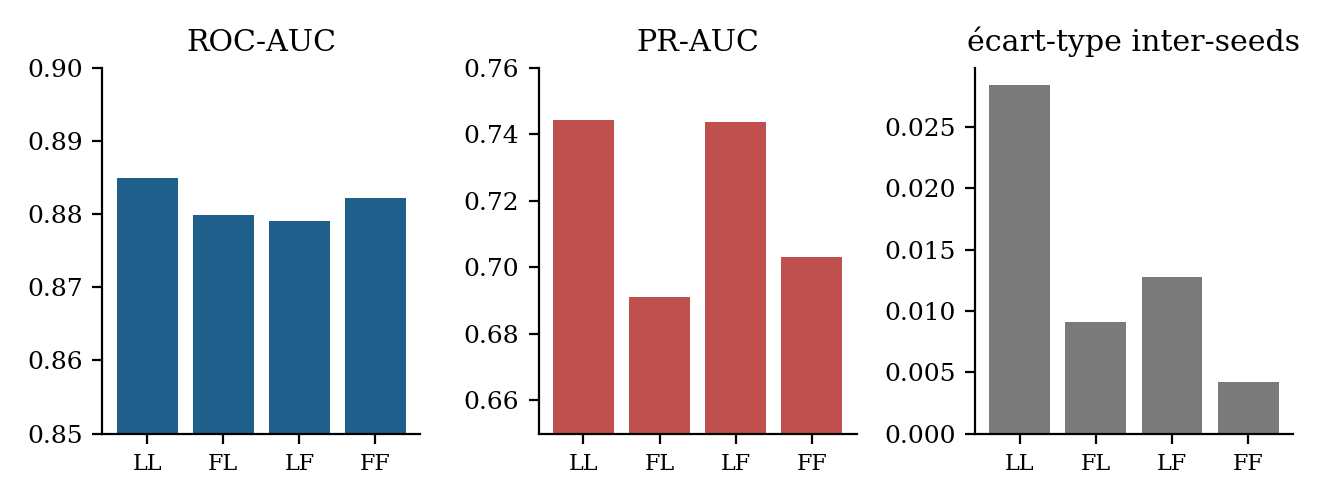
\includegraphics[width=0.96\textwidth]{figures/14_mechanism.png}
\caption{Ablation des mécanismes, quatre branches. L~: appris par jour~; F~: figé à un scalaire appris.}
\label{fig:mechanism}
\end{figure}

\begin{table}[htbp]
\centering\small
\caption{Ablation des mécanismes, moyennes sur six plis, cinq graines. Nombre de paramètres avec $d=4$.}
\label{tab:mechanism}
\begin{tabular}{lccccccc}
\toprule
Branche & Paramètres & ROC-AUC & PR-AUC & F1 & ECE & Transition-AUC & $\sigma_{\text{graines}}$ \\
\midrule
LL & 31\,381 & 0,885 & \textbf{0,744} & 0,621 & 0,107 & 0,816 & 0,028 \\
FL & 28\,692 & 0,880 & 0,691 & 0,566 & 0,128 & \textbf{0,836} & 0,009 \\
LF & 23\,317 & 0,879 & \textbf{0,744} & \textbf{0,622} & \textbf{0,096} & 0,792 & 0,013 \\
FF & 20\,628 & 0,882 & 0,703 & 0,580 & 0,119 & 0,831 & \textbf{0,004} \\
\bottomrule
\end{tabular}
\end{table}

Le tableau~\ref{tab:mechanism} et la figure~\ref{fig:mechanism} donnent le résultat, et il faut le lire en deux temps.

Sur le ROC-AUC, FF égale LL~: $0{,}882$ contre $0{,}885$, et sur les six plis un seul écart dépasse le bruit inter-graines --- le pli 4, encore. Geler l'ensemble des paramètres physiques à six constantes ne coûte rien sur le classement des jours. C'est le troisième scénario de la grille, celui que nous redoutions, et nous devons en tirer la conséquence~: l'affirmation qu'un potentiel appris jour par jour \emph{classe mieux} qu'un potentiel fixe n'est pas soutenue par nos données. Ce que nous avions annoncé dans les versions antérieures de ce travail doit être retiré.

Sur le PR-AUC et le F1, en revanche, LL bat FF de $0{,}041$ sur chacun, et cet écart est porté principalement par le pli 4, où FL --- puits figé --- s'effondre ($-0{,}061$ en ROC-AUC, PR-AUC de $0{,}350$ à $0{,}266$), seul pli où le puits figé échoue. La formulation honnête devient donc~: \emph{la modulation journalière du potentiel n'améliore pas le classement général~; elle améliore la précision sur la classe crise, et elle est nécessaire pour une crise sur six.} C'est plus étroit que ce que nous pensions. C'est ce que les données disent.

Deux résultats de cette ablation valent davantage que le verdict lui-même. Le premier est que la variance inter-graines s'effondre à chaque gel~: $0{,}028$ pour LL, $0{,}013$ pour LF, $0{,}009$ pour FL, $0{,}004$ pour FF. L'encodeur lent, qui produit le potentiel, est la source dominante de l'instabilité qui a limité toutes nos comparaisons. Le second est que les scalaires vers lesquels FF converge sont remarquablement stables sur les six fenêtres d'entraînement~: $\dV = 0{,}32$ à $0{,}33$, $\gamma = 0{,}47$, $T = 0{,}058$. Nous discuterons en section~\ref{sec:discussion} ce que cette stabilité signifie et ce qu'elle ne signifie pas.

Enfin, LF --- potentiel appris, thermostat figé --- présente la meilleure calibration des quatre branches (ECE $0{,}096$), le meilleur pli 4 (ROC-AUC $0{,}862$, PR-AUC $0{,}413$, contre $0{,}833$ et $0{,}350$ pour LL), un PR-AUC et un F1 égaux à LL, et une variance inter-graines deux fois plus faible. Le thermostat appris était donc ce qui dégradait la calibration. LF est, de ce fait, un candidat sérieux pour remplacer l'architecture complète, et nous le reprenons en section~\ref{sec:final}.

\subsection{Jusqu'où soustraire}
\label{sec:minimal}

FF apprend encore une chose par jour~: l'encodeur rapide, cinq petits réseaux produisant l'état initial, la force externe et la mémoire. Deux branches demandent s'il a besoin d'être non linéaire, et s'il a besoin de 124 descripteurs~:
\begin{itemize}\setlength\itemsep{0pt}
\item \textbf{FF$_\mathrm{lin}$}~: FF avec chaque réseau de l'encodeur remplacé par une application linéaire --- 1\,916 paramètres~;
\item \textbf{FF$_\mathrm{vol}$}~: FF$_\mathrm{lin}$ restreint aux 40 descripteurs de volatilité --- 740 paramètres.
\end{itemize}
La seconde met à l'épreuve, à pleine échelle, l'ablation par groupe de la section~\ref{sec:audit}.

\begin{figure}[htbp]
\centering
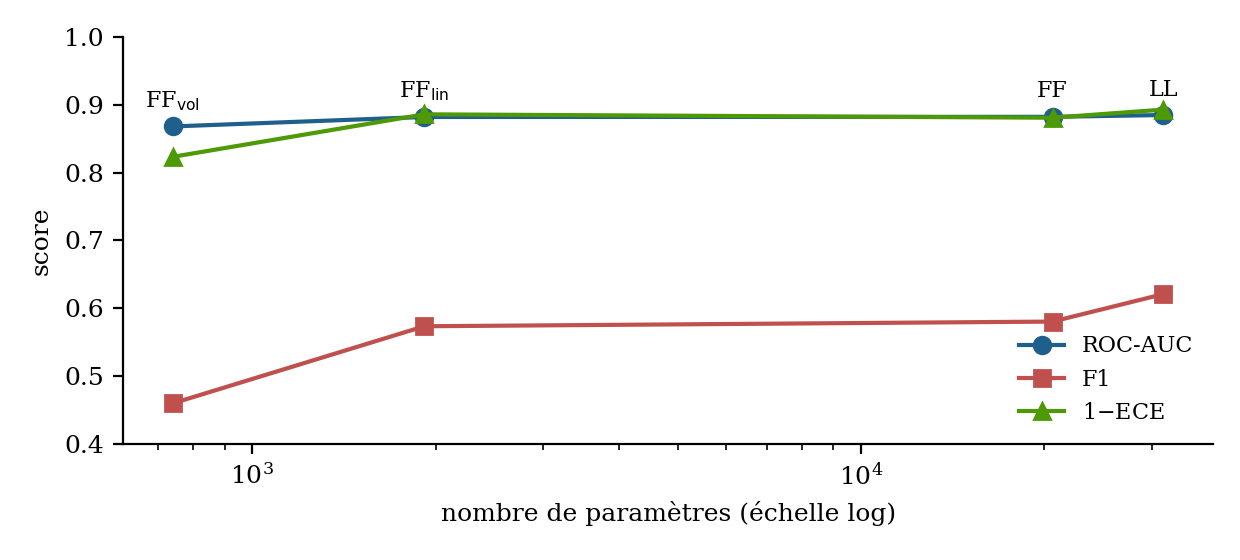
\includegraphics[width=0.84\textwidth]{figures/15_parsimony.png}
\caption{La chaîne de soustraction. Le ROC-AUC se maintient jusqu'à 740 paramètres~; le F1 et la calibration cèdent avant.}
\label{fig:parsimony}
\end{figure}

La figure~\ref{fig:parsimony} montre où la chaîne casse. FF$_\mathrm{lin}$ égale FF sur le ROC-AUC ($0{,}882$ contre $0{,}882$, cinq plis sur six dans le bruit) avec seize fois moins de paramètres~: la non-linéarité de l'encodeur est décorative. Mais la barrière figée, qui était plate à $0{,}32\pm0{,}003$ dans FF, \emph{dérive} de $0{,}283$ à $0{,}248$ à travers les six fenêtres dans FF$_\mathrm{lin}$. L'encodeur non linéaire absorbait quelque chose que la version linéaire reporte sur le scalaire. Le résultat de parcimonie tient~; celui de constante stable ne survit pas à cette simplification-là.

FF$_\mathrm{vol}$ casse, et le ROC-AUC seul le cachait. Il se maintient à $0{,}868$, mais le F1 tombe de $0{,}621$ à $0{,}460$ et l'ECE monte de $0{,}107$ à $0{,}177$, avec $0{,}288$ sur le pli 3 et $0{,}246$ sur le pli 4 --- parmi les pires chiffres de calibration de tout ce travail. Le ROC-AUC ne mesure que le classement~; la volatilité seule sait dire \og quelque chose se passe \fg{} et classe correctement, mais elle ne sait pas dire \og c'est une crise, avec cette confiance \fg{}. Pli par pli, la restriction améliore les deux crises où un pic de volatilité suffit (2011, COVID) et dégrade les trois autres au-delà du bruit. Le modèle a besoin d'autre chose que de volatilité, et c'est cette autre chose qui porte la calibration.

\subsection{Le pli 4}
\label{sec:fold4}

Le quatrième trimestre 2018 apparaît comme singulier dans quatre expériences indépendantes~: c'est le seul pli où le terme de brisure de symétrie structuré améliore franchement la détection précoce (section~\ref{sec:tilt}), le seul où le puits figé échoue (section~\ref{sec:mechanism}), celui où le thermostat figé fait le mieux, et le pire pour FF$_\mathrm{vol}$. Ce n'est pas une coïncidence~; c'est un fait sur les données. L'épisode d'octobre--décembre 2018 est une correction rapide, d'environ vingt pour cent, suivie d'un rebond en V, déclenchée par des craintes sur les taux et le commerce plutôt que par un choc de liquidité. Elle a, de toutes nos crises, la signature de volatilité la plus faible relativement à sa profondeur. Un détecteur de volatilité la voit mal~; un terme de tendance la voit mieux~; un puits qui se déforme la voit mieux encore. La physique modulée jour par jour n'est pas nécessaire aux crises que la volatilité annonce. Elle est nécessaire à celle que la volatilité n'annonce pas.

\FloatBarrier
\section{Lire la physique~: des signaux au-delà de la tête de sortie}
\label{sec:physics}

Le modèle produit chaque jour, outre $\Psiv$, un état $(\mathbf z_N,\mathbf p_N)$ et des paramètres $(a,b,\gamma,T)$. La tête de lecture n'en extrait qu'une projection. Nous avons demandé si ces quantités, lues par la physique plutôt que par un réseau, portent une information que $\Psiv$ ne porte pas. Tout ce qui suit est calculé \emph{après} entraînement, à partir de modèles déjà entraînés~: aucun degré de liberté n'est ajouté, et le risque qui a fait échouer nos quatre extensions rejetées n'existe pas ici.

\subsection{Le régime de friction}

Le taux d'échappement de Kramers~\cite{kramers1940} dépend du régime de friction, et nos versions antérieures utilisaient sa forme haute friction en admettant que la friction apprise pouvait traverser le point de retournement. Pour le potentiel~\eqref{eq:potential}, la courbure au fond du puits donne $\omega_0 = 2\sqrt b$ et celle de la barrière $\omega_b = \sqrt{2b}$~; la friction continue est $\Gamma = \gamma/\delta t$. Le régime est fixé par $\Gamma/\omega_b$. Sur les données réelles, la fraction de jours en basse friction ($\Gamma/\omega_b < 1$) est \emph{nulle} sur cinq plis et de trois pour cent sur le sixième. L'hypothèse haute friction est correcte sur l'ensemble de l'échantillon~; une limite que nous avions déclarée se referme.

\subsection{Le taux de Kramers avec ses préfacteurs}

Nous avons calculé quatre proxys de taux~: la forme brute $\gamma^{-1}e^{-\dV/T}$ utilisée jusqu'ici, la forme de diffusion spatiale avec préfacteurs de courbure~\cite{hanggi1990}, la forme de diffusion d'énergie (basse friction), et un pont harmonique entre les deux. Aucun n'est un taux en unités calendaires~; tous sont des proxys de rang, mais des proxys \emph{différents}, parce que les préfacteurs dépendent de $(a,b,\gamma)$ d'une manière qui ne se réduit pas à une transformation monotone de la forme brute.

Comme détecteur autonome, le meilleur est la forme d'énergie ($0{,}850$ de ROC-AUC contre $0{,}831$ pour la forme brute, sur chacun des six plis) --- résultat curieux, puisque c'est la formule du mauvais régime, dont le préfacteur linéaire en $\dV/T$ fait visiblement un travail que l'exponentielle seule ne fait pas. Nous le rapportons comme un meilleur proxy de rang, sans lui prêter de justification physique propre.

Un point doit être dit clairement. Le taux brut, tel que nous le calculons à partir de la barrière non inclinée, est \emph{anti-corrélé} à la crise sur chacun des six plis, de façon parfaitement stable. Le signe est donc fixé sur les données d'entraînement et n'est pas un problème pratique. Mais nos versions antérieures affirmaient que $T$ monte, que $\gamma$ baisse et que $\dV$ baisse en crise, trois corrélations qui, combinées dans $\gamma^{-1}e^{-\dV/T}$, imposent un taux qui \emph{monte}. L'une des trois affirmations, ou leur combinaison, ne tient pas telle qu'elle était écrite, et la question de savoir de quel puits ce taux mesure l'échappement reste ouverte. Nous préférons le signaler que de l'attribuer à une erreur de convention.

\subsection{Complémentarité au début des crises}

La figure~\ref{fig:onset} montre la Transition-AUC de $\Psiv$ et des signaux physiques, pli par pli. Ils ne ratent pas les mêmes crises. Sur le pli 3 (2015), $\Psiv$ est au hasard au démarrage ($0{,}547$) et le taux de Kramers est presque parfait ($0{,}993$)~; sur le pli 1 (2008), c'est l'inverse. Sur le pli 4, la violation de fluctuation--dissipation $\Delta_{\mathrm{FDT}} = \lvert\,\lVert\mathbf p_N\rVert^2/d - T\,\rvert$, mesure de la distance à l'équipartition inspirée de la littérature des températures effectives~\cite{cugliandolo1997}, atteint $0{,}982$ là où $\Psiv$ fait $0{,}745$. C'est précisément cette complémentarité qui rend un ensemble utile.

\begin{figure}[htbp]
\centering
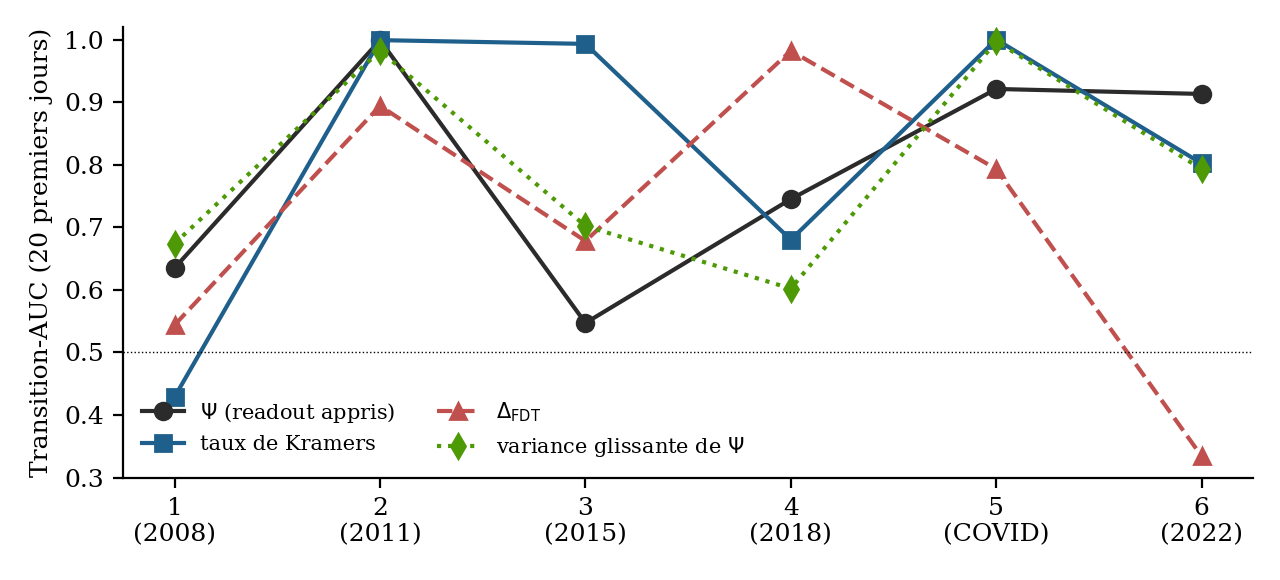
\includegraphics[width=0.9\textwidth]{figures/16_onset.png}
\caption{Transition-AUC par pli pour la jauge apprise et trois signaux physiques calculés après entraînement. Les signaux ne défaillent pas sur les mêmes plis.}
\label{fig:onset}
\end{figure}

Nous devons cependant être précis sur $\Delta_{\mathrm{FDT}}$. Son ROC-AUC moyen de $0{,}754$ cache une instabilité~: son signe s'inverse sur deux plis sur six, et il est proche du hasard sur les plis 1 et 6. L'hypothèse \og la violation de la FDT est un signal précurseur \fg{} n'est pas soutenue proprement. Nous la rapportons comme un résultat négatif, et nous ne l'utilisons pas dans l'ensemble final.

\subsection{Vacillement}

La littérature des transitions critiques propose, pour un système bistable dont le puits ne s'aplatit pas, un signal précurseur différent du ralentissement~: le vacillement, visible dans la variance du paramètre d'ordre sur une fenêtre glissante~\cite{wang2012,dakos2013}. $\Psiv$ étant le paramètre d'ordre que le modèle définit lui-même, nous avons calculé sa variance glissante sur 20 jours, et son taux de croisement de la médiane glissante. La variance porte un signal réel --- ROC-AUC $0{,}774$, au-dessus du hasard sur chacun des six plis --- et surtout \emph{son signe ne s'inverse jamais}~: la variance monte quand la crise approche, dans le sens que la théorie prédit, sur les six plis. Le taux de croisement, lui, est faible ($0{,}577$) et instable (quatre inversions sur six). Dakos \emph{et al.} avaient raison de préférer la variance comme opérationnalisation~; nos deux résultats le confirment dans les deux sens.

\subsection{L'ensemble final}
\label{sec:final}

Une régression logistique combinant $\Psiv$ et le taux de Kramers, essayée dans une version antérieure, n'avait pas battu $\Psiv$ seul~: la queue de calibration ne contient qu'un épisode, trop peu pour ajuster deux poids. Une moyenne de rangs n'a aucun poids à ajuster. Elle exige seulement d'orienter chaque signal, et nous l'orientons sur la fenêtre d'entraînement \emph{complète} plutôt que sur la queue de calibration --- celle-ci ne contient aucun jour de crise sur trois plis, ce qui avait limité tous nos résultats d'ensemble antérieurs à trois plis sur six, alors que la fenêtre complète en contient cinq cents ou plus sur chacun. L'orientation est un bit par signal, non une température~; elle n'a pas besoin d'être récente, elle a besoin d'être stable, et les deux signes le sont.

\begin{figure}[t]
\centering
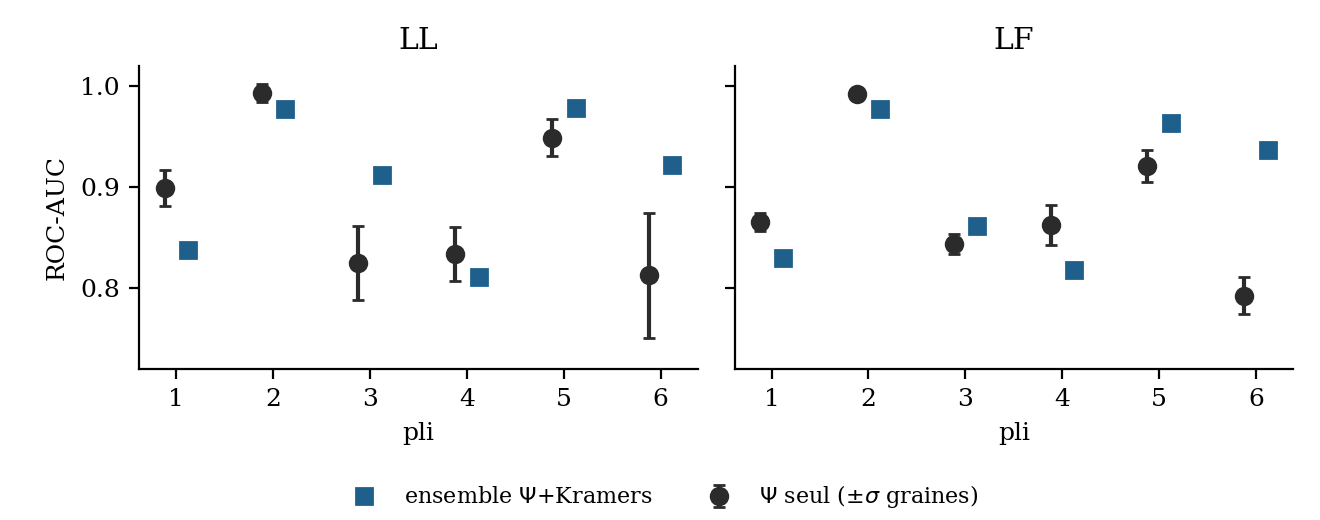
\includegraphics[width=0.94\textwidth]{figures/17_final_ensemble.png}
\caption{ROC-AUC par pli, jauge seule (avec barre d'écart-type inter-graines) et ensemble de rangs $\Psiv$+Kramers, pour l'architecture complète (LL) et pour LF.}
\label{fig:final}
\end{figure}

\begin{table}[htbp]
\centering\small
\caption{Ensemble de rangs, six plis sur six, orientation sur la fenêtre d'entraînement complète. Ensemble à deux~: $\Psiv$ et taux de Kramers~; à trois~: plus la variance glissante de $\Psiv$.}
\label{tab:final}
\begin{tabular}{llcccc}
\toprule
Architecture & Lecture & ROC-AUC & PR-AUC & Transition-AUC & $\sigma_{\text{graines}}$ \\
\midrule
\multirow{3}{*}{LL} & $\Psiv$ seul & 0,885 & 0,745 & 0,818 & \multirow{3}{*}{0,028} \\
 & ensemble à deux & \textbf{0,906} & \textbf{0,748} & 0,854 & \\
 & ensemble à trois & 0,896 & 0,675 & \textbf{0,864} & \\
\midrule
\multirow{3}{*}{LF} & $\Psiv$ seul & 0,879 & 0,744 & 0,792 & \multirow{3}{*}{\textbf{0,013}} \\
 & ensemble à deux & 0,898 & \textbf{0,748} & \textbf{0,865} & \\
 & ensemble à trois & 0,872 & 0,604 & 0,848 & \\
\bottomrule
\end{tabular}
\end{table}

Le tableau~\ref{tab:final} et la figure~\ref{fig:final} donnent le résultat sur les six plis, et il corrige une estimation antérieure. Sur trois plis, nous avions mesuré un gain de $+0{,}030$~; sur six, il est de $+0{,}021$ pour LL et $+0{,}018$ pour LF --- l'échantillon à trois plis était biaisé vers ceux où l'ensemble aide. Et il n'aide pas partout~: il dégrade les plis 1 et 2, au-delà du bruit, là où $\Psiv$ seul était déjà excellent ($0{,}99$ sur le pli 2), et il améliore substantiellement les plis 3, 5 et 6, là où $\Psiv$ seul peine ($+0{,}087$ et $+0{,}109$ sur les plis 3 et 6 pour LL). Adopter l'ensemble est un échange, non un gain gratuit.

Sur la Transition-AUC, en revanche, le gain est net et cohérent~: $+0{,}035$ pour LL, $+0{,}073$ pour LF. Ce n'est pas surprenant~: un taux d'échappement est par construction une mesure de proximité au basculement, non de position dans l'épisode, et c'est au début des crises qu'il complète le mieux la jauge apprise.

L'ensemble à trois, ajoutant la variance glissante, est confirmé inférieur à l'ensemble à deux sur les données complètes~: il dégrade fortement les plis 2 et 5. Un signal plus faible, moyenné à poids égal avec un ensemble déjà bon, le dilue. La variance de $\Psiv$ est un vrai signal~; elle n'est pas un troisième composant de cet ensemble.

Entre LL et LF, le choix reste ouvert et nous le disons. LL fait mieux en moyenne, mais cet écart ne dépasse le bruit inter-graines que sur un seul pli, le troisième. LF est deux fois plus stable et un tiers plus léger. Nous retenons LL avec l'ensemble à deux comme chiffre principal --- ROC-AUC $0{,}906$, Transition-AUC $0{,}854$, six plis --- parce que c'est l'architecture que cet article décrit, et nous présentons LF comme l'alternative plus sobre, de performance équivalente au bruit près.

\section{Discussion~: le puits ne bouge pas, le système vacille}
\label{sec:discussion}

Trois observations indépendantes pointent dans le même sens. Guttal \emph{et al.}~\cite{guttal2016} n'ont trouvé aucune montée de l'autocorrélation avant les krachs américains, mais une montée de la variance. Notre ablation des mécanismes montre qu'un puits figé suffit à cinq crises sur six~: le paysage n'a pas besoin de se déformer pour que le modèle détecte la transition. Et la variance glissante de notre propre jauge porte un signal dont le signe ne s'inverse jamais, exactement ce que la théorie du vacillement~\cite{wang2012,dakos2013} prédit pour un système bistable sous fort bruit. Aucune des trois n'est décisive seule. Ensemble, elles constituent une position dans un débat ouvert~: dans la mesure où nos données en témoignent, les crises de marché ne sont pas des bifurcations au sens de Scheffer, elles sont des transitions stochastiques --- le puits reste, le bruit pousse.

Ceci reformule ce que le modèle est. Nous l'avions décrit comme un potentiel appris jour par jour~; il est mieux décrit comme un paysage essentiellement \emph{fixe}, dans lequel ce qui varie est la position de départ et la force qui pousse. Les six constantes vers lesquelles FF converge --- $\dV\approx0{,}32$, $\gamma\approx0{,}47$, $T\approx0{,}058$ --- sont retrouvées sur six fenêtres d'entraînement, et nous avons d'abord voulu y voir des constantes du marché. Nous devons être plus prudents. Les fenêtres sont emboîtées, non indépendantes~: le pli 6 contient toutes les données du pli 1. Une part de cette stabilité peut être mécanique. Un indice qu'elle ne l'est pas entièrement est que FF$_\mathrm{lin}$, sous les mêmes fenêtres emboîtées, produit une barrière qui \emph{dérive}~: si la stabilité était un artefact des fenêtres, elle se verrait aussi là. Mais ce n'est qu'un indice, et le seul test qui trancherait --- le même pipeline sur un marché différent --- n'a pas été fait.

Ce que le modèle apprend jour par jour n'est pas rien, mais c'est moins que ce que nous pensions, et c'est localisé. La modulation du potentiel porte la précision sur la classe crise et elle porte le pli 4, cette correction de 2018 que la volatilité n'annonce pas. Le thermostat appris, lui, dégrade la calibration et peut être figé. Le terme de brisure de symétrie tient en un scalaire et une forme empruntée à Chiarella. L'encodeur peut être linéaire. Neuf modifications de l'architecture --- quatre extensions rejetées, deux lignées abandonnées, et les trois branches ajoutant de la liberté dans ce travail --- n'ont produit aucun gain~; trois lectures différentes du modèle existant en ont produit chacune un. Sur ce projet, le motif est sans ambiguïté~: ce qui a marché est venu de mieux lire, non de reconstruire.

\section{Ce que nous ne savons pas}
\label{sec:limits}

Six fenêtres de test, treize épisodes datés à la main, un seul marché. Aucune affirmation statistique forte n'est possible sur cette base, et nous avons essayé de n'en faire aucune~; là où nous avons échoué dans les versions antérieures, nous l'avons dit. Les fenêtres d'entraînement sont emboîtées, ce qui affaiblit toute lecture de \og réplication \fg{}. L'écart-type inter-graines, que nous avons enregistré partout, est sur certains plis plus grand que la plupart des effets~; c'est lui qui a rendu \og dans le bruit \fg{} la majorité de nos comparaisons, et c'est une limite du modèle complet plus que de la mesure --- ses variantes figées ne l'ont pas. La règle de tendance nous devance sur le ROC-AUC. Le calendrier d'entraînement dépasse l'optimum. L'interprétation physique du signe du taux de Kramers est incomplète. La Transition-AUC n'a pas été enregistrée par graine, et ses gains les plus frappants --- le pli 4 --- ne sont pas certifiés contre le bruit. Le cadre log-périodique de Sornette n'a pas été comparé. Le test sur un autre marché, qui répondrait à la fois à la question de la généralisation et à celle de la constante, n'a pas été fait, et c'est la première chose à faire.

\section{Conclusion}

Nous avons construit un détecteur de crises autour d'un mécanisme physique, puis nous avons cherché à savoir quelle part de ce mécanisme était nécessaire. La réponse est~: moins que nous ne le pensions, mais pas rien, et pas là où nous le pensions. Le classement des jours ne dépend presque pas de la physique apprise~; la précision et la détection d'une crise particulière en dépendent. Le paysage énergétique est essentiellement fixe. Ce qu'il y a de plus utile dans le modèle n'est pas sa tête de sortie mais ce qu'on peut lire de son état par la théorie des taux de réaction et par la variance de sa jauge, en particulier au moment où une crise commence. Et ce que l'ensemble suggère sur le mécanisme des crises --- le vacillement plutôt que le ralentissement --- rejoint ce que d'autres ont observé par d'autres moyens. Nous livrons ces résultats avec leurs limites, parce qu'un résultat mitigé rapporté honnêtement vaut plus qu'un résultat flatteur obtenu en cherchant jusqu'à ce qu'il sorte.

\paragraph{Reproductibilité.} Le code du modèle, les scripts de chaque ablation, les résultats bruts par pli et par graine et la source de cet article sont disponibles dans le dossier \texttt{reproducibility/} du dépôt \url{https://github.com/Ahmed-Hadirassou/PhaseIndexDetector-SingleParticle}, avec une table de correspondance entre chaque tableau ou figure et le script qui le produit.

\paragraph{Usage d'outils d'intelligence artificielle.} Ce travail a été mené avec l'assistance d'un modèle de langage (Claude, Anthropic). Il a été utilisé pour concevoir et écrire les scripts d'ablation et d'évaluation, pour analyser les résultats au fur et à mesure, et pour rédiger le présent texte. L'architecture du modèle, le choix des hypothèses à tester, l'exécution de tous les calculs, la vérification des résultats et la responsabilité des affirmations qui précèdent sont de l'auteur. Chaque référence bibliographique a été vérifiée individuellement. Nous le signalons parce que nous pensons que la manière dont un résultat est obtenu fait partie du résultat.

\begin{thebibliography}{99}\small

\bibitem{bollerslev1986}
T. Bollerslev, \emph{Generalized autoregressive conditional heteroskedasticity}, J. Econometrics \textbf{31}(3), 307--327 (1986).

\bibitem{bouchaud1998}
J.-P. Bouchaud et R. Cont, \emph{A Langevin approach to stock market fluctuations and crashes}, Eur. Phys. J. B \textbf{6}, 543--550 (1998).

\bibitem{chiarella1992}
C. Chiarella, \emph{The dynamics of speculative behaviour}, Ann. Oper. Res. \textbf{37}, 101--123 (1992).

\bibitem{cugliandolo1997}
L. F. Cugliandolo, J. Kurchan et L. Peliti, \emph{Energy flow, partial equilibration, and effective temperatures in systems with slow dynamics}, Phys. Rev. E \textbf{55}, 3898 (1997).

\bibitem{dakos2013}
V. Dakos, E. H. van Nes et M. Scheffer, \emph{Flickering as an early warning signal}, Theor. Ecol. \textbf{6}, 309--317 (2013).

\bibitem{diks2019}
C. Diks, C. Hommes et J. Wang, \emph{Critical slowing down as an early warning signal for financial crises?}, Empir. Econ. \textbf{57}, 1201--1228 (2019).

\bibitem{faber2007}
M. T. Faber, \emph{A quantitative approach to tactical asset allocation}, J. Wealth Manag. \textbf{9}(4), 69--79 (2007).

\bibitem{gelman2013}
A. Gelman et E. Loken, \emph{The garden of forking paths: why multiple comparisons can be a problem, even when there is no ``fishing expedition'' or ``p-hacking'' and the research hypothesis was posited ahead of time}, manuscrit, Columbia University (2013).

\bibitem{guo2017}
C. Guo, G. Pleiss, Y. Sun et K. Q. Weinberger, \emph{On calibration of modern neural networks}, Proc. ICML (2017).

\bibitem{guttal2016}
V. Guttal, S. Raghavendra, N. Goel et Q. Hoarau, \emph{Lack of critical slowing down suggests that financial meltdowns are not critical transitions, yet rising variability could signal systemic risk}, PLoS ONE \textbf{11}(1), e0144198 (2016).

\bibitem{halperin2019}
I. Halperin et M. Dixon, \emph{``Quantum equilibrium-disequilibrium'': asset price dynamics, symmetry breaking, and defaults as dissipative instantons}, Physica A \textbf{537}, 122187 (2019).

\bibitem{hamilton1989}
J. D. Hamilton, \emph{A new approach to the economic analysis of nonstationary time series and the business cycle}, Econometrica \textbf{57}(2), 357--384 (1989).

\bibitem{hanggi1990}
P. H\"anggi, P. Talkner et M. Borkovec, \emph{Reaction-rate theory: fifty years after Kramers}, Rev. Mod. Phys. \textbf{62}, 251--341 (1990).

\bibitem{johansen1999}
A. Johansen, O. Ledoit et D. Sornette, \emph{Predicting financial crashes using discrete scale invariance}, J. Risk \textbf{1}, 5--32 (1999).

\bibitem{kramers1940}
H. A. Kramers, \emph{Brownian motion in a field of force and the diffusion model of chemical reactions}, Physica \textbf{7}(4), 284--304 (1940).

\bibitem{kurth2025chiarella}
J. G. Kurth et J.-P. Bouchaud, \emph{Stationary distributions of the mode-switching Chiarella model}, arXiv:2511.13277 (2025).

\bibitem{kurth2025excess}
J. G. Kurth, A. A. Majewski et J.-P. Bouchaud, \emph{Revisiting the excess volatility puzzle through the lens of the Chiarella model}, arXiv:2505.07820 (2025).

\bibitem{majewski2020}
A. A. Majewski, S. Ciliberti et J.-P. Bouchaud, \emph{Co-existence of trend and value in financial markets: estimating an extended Chiarella model}, J. Econ. Behav. Organ. \textbf{174}, 1--15 (2020).

\bibitem{mori1965}
H. Mori, \emph{Transport, collective motion, and Brownian motion}, Prog. Theor. Phys. \textbf{33}, 423--455 (1965).

\bibitem{moskowitz2012}
T. J. Moskowitz, Y. H. Ooi et L. H. Pedersen, \emph{Time series momentum}, J. Financ. Econ. \textbf{104}(2), 228--250 (2012).

\bibitem{perretti2012}
C. T. Perretti et S. B. Munch, \emph{Regime shift indicators fail under noise levels commonly observed in ecological systems}, Ecol. Appl. \textbf{22}(6), 1772--1779 (2012).

\bibitem{rinn2015}
P. Rinn, Y. Stepanov, J. Peinke, T. Guhr et R. Sch\"afer, \emph{Dynamics of quasi-stationary systems: finance as an example}, EPL \textbf{110}, 68003 (2015).

\bibitem{saito2015}
T. Saito et M. Rehmsmeier, \emph{The precision-recall plot is more informative than the ROC plot when evaluating binary classifiers on imbalanced datasets}, PLoS ONE \textbf{10}(3), e0118432 (2015).

\bibitem{sandhu2016}
R. S. Sandhu, T. T. Georgiou et A. R. Tannenbaum, \emph{Ricci curvature: an economic indicator for market fragility and systemic risk}, Sci. Adv. \textbf{2}(5), e1501495 (2016).

\bibitem{scheffer2009}
M. Scheffer, J. Bascompte, W. A. Brock, V. Brovkin, S. R. Carpenter, V. Dakos, H. Held, E. H. van Nes, M. Rietkerk et G. Sugihara, \emph{Early-warning signals for critical transitions}, Nature \textbf{461}, 53--59 (2009).

\bibitem{sornette2003}
D. Sornette, \emph{Why Stock Markets Crash: Critical Events in Complex Financial Systems}, Princeton University Press (2003).

\bibitem{topological2025}
E. Guritanu, E. Barbierato et A. Gatti, \emph{Topological machine learning for financial crisis detection: early warning signals from persistent homology}, Computers \textbf{14}(10), 408 (2025).

\bibitem{verlet1967}
L. Verlet, \emph{Computer ``experiments'' on classical fluids. I. Thermodynamical properties of Lennard-Jones molecules}, Phys. Rev. \textbf{159}, 98--103 (1967).

\bibitem{wand2024}
T. Wand, T. Wiedemann, J. Harren et O. Kamps, \emph{Estimating stable fixed points and Langevin potentials for financial dynamics}, Phys. Rev. E \textbf{109}, 024226 (2024).

\bibitem{wang2012}
R. Wang, J. A. Dearing, P. G. Langdon, E. Zhang, X. Yang, V. Dakos et M. Scheffer, \emph{Flickering gives early warning signals of a critical transition to a eutrophic lake state}, Nature \textbf{492}, 419--422 (2012).

\bibitem{whaley2000}
R. E. Whaley, \emph{The investor fear gauge}, J. Portf. Manag. \textbf{26}(3), 12--17 (2000).

\bibitem{zwanzig1961}
R. Zwanzig, \emph{Memory effects in irreversible thermodynamics}, Phys. Rev. \textbf{124}, 983--992 (1961).

\end{thebibliography}

\end{document}
